\documentclass[usenames,dvipsnames,tikz]{standalone}
\usetikzlibrary{patterns}
%\usepackage{amsmath,amssymb}
%\usepackage{xcolor}
\colorlet{tBlue}{RoyalBlue!35!Cerulean}
\colorlet{tRed}{Red}
%\usepackage{tikz}
%\usepackage{standalone}
\definecolor{tLightOrange}{HTML}{FFE3B2}
\definecolor{tLightGreen}{HTML}{D3ECAA}
\definecolor{tLightPink}{HTML}{FFD4EB} %tikz color
\definecolor{tLightBlue}{HTML}{CEF0FF} %tikz color
\definecolor{tLightYellow}{HTML}{FFFBBD} %tikz color
\definecolor{tLightPurple}{HTML}{ECDBFF} %tikz color
\begin{document}
	
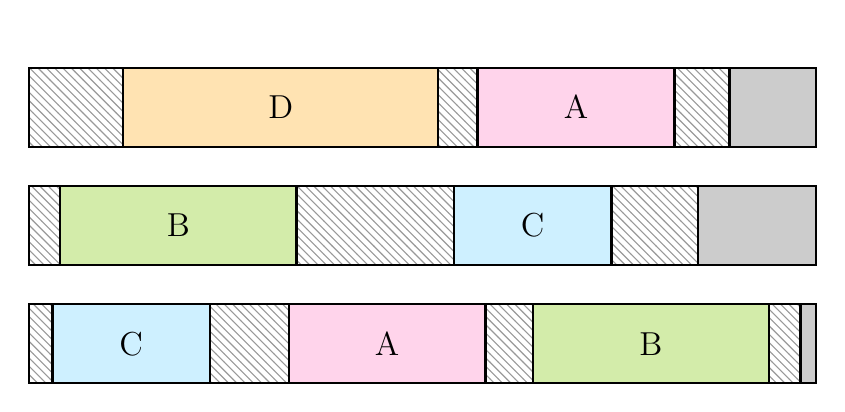
\begin{tikzpicture}
%\draw [help lines] (-1,-2) grid (11,5);

%--------------------------------

\draw [thick, white] (0,4.5) -- (10,4.5);

% SDCL, lined area shows inter item waste
%Top row
\draw [thick, pattern = north west lines, pattern color=black!40!white] (0,3) rectangle (10,4);
\draw [thick, fill=tLightOrange] (1.2,3) rectangle (5.2,4);
\draw [thick, fill=tLightPink] (5.7,3) rectangle (8.2,4);
\draw [thick, fill=black!20!white] (8.9,3) rectangle (10,4);
\node at (3.2, 3.5) {\large D};
\node at (6.95, 3.5) {\large A};

%Middle row
\draw [thick, pattern = north west lines, pattern color=black!40!white] (0,1.5) rectangle (10,2.5);
\draw [thick, fill=tLightGreen] (0.4,1.5) rectangle (3.4,2.5);
\draw [thick, fill=tLightBlue] (5.4,1.5) rectangle (7.4,2.5);
\draw [thick, fill=black!20!white] (8.5,1.5) rectangle (10,2.5);
\node at (1.9, 2) {\large B};
\node at (6.4, 2) {\large C};

%Bottom row
\draw [thick, pattern = north west lines, pattern color=black!40!white] (0,0) rectangle (10,1); 
\draw [thick, fill=tLightBlue] (0.3,0) rectangle (2.3,1);
\draw [thick, fill=tLightPink] (3.3,0) rectangle (5.8,1);
\draw [thick, fill=tLightGreen] (6.4,0) rectangle (9.4,1);
\draw [thick, fill=black!20!white] (9.8,0) rectangle (10,1);
\node at (1.3, 0.5) {\large C};
\node at (4.55, 0.5) {\large A};
\node at (7.9, 0.5) {\large B};
%\filldraw[fill=black!20!white, draw=black, thick] (8.8,1) -- (8.8,0) -- (10,0) -- (10,1) -- (8.8,1);


%\filldraw[fill=white, draw=black, thick] (0,1) -- (1,0) -- (2,0) -- (2.3,1) -- (0,1);
%\filldraw[fill=white, draw=black, thick] (2.3,1) -- (2.2,0) -- (3.5,0) -- (3.1,1) -- (2.3,1);
%\filldraw[fill=white, draw=black, thick] (3.1,1) -- (3.5,0) -- (4.7,0) -- (5.2,1) -- (3.1,1);
%\filldraw[fill=white, draw=black, thick] (5.2,1) -- (4.7,0) -- (6.7,0) -- (7.2,1) -- (5.2,1);
%\filldraw[fill=white, draw=black, thick] (7.2,1) -- (7,0) -- (8.8,0) -- (8.3,1) -- (7.2,1);


\end{tikzpicture}

\end{document}